 \subsection{Régression Logistique  }
 La régression logistique est une technique de classification , elle consiste à appliquer une fonction h sur des éléments ${x}_{1}$ ,${x}_{2}$,${x}_{3}$ .... ${x}_{n}$ en entrée et trouver une sortie \emph{discrète} y. \\
 Cette sortie nous permet de déterminer la classe du tuple , généralement y prend 2 valeurs 0 ou 1 et quelque fois -1  ou 1.\\
 On utilise ce type de classification dans différents cas :

 - Classification des emails : spams ou non spam

 - Transaction en Ligne : Frauduleux ou pas

 - Crédit bancaire : risquant ou non

 - Tumeur : Bénigne ou Maligne

\subsubsection{Représentation de l'hypothèse}
Une première approche serait d'utiliser la régression linéaire avec la fonction ${h}_{\theta}\left(x\right)={\theta }_{0}{x}_{0}+{\theta }_{1}{x}_{1}+{\theta }_{2}{x}_{2}+{\theta }_{3}{x}_{3}+....{\theta }_{n}{x}_{n}$  pour effectuer la classification mais cela peut un problème car ${h}_{\theta}\left(x\right)$ peut prendre des valeur qui sont à l'extérieur de  l'intervalle [0,1].
La meilleur solution serait de trouver une fonction qui ne prend que des valeurs comprises entre 0 et 1 .

Pour les problèmes de classification on utilise la fonction sigmoïde ,elle est définie par :

\begin{center}
	$g(z) =\frac{1}{1+{e}^{-z}}$
\end{center}
Et ainsi notre hypothèse sera :
\begin{center}
	${h}_{\theta}\left(x\right)=g({\theta }^{T}{x})$
\end{center}
Avec ${\theta }^{T}{x}={\theta }_{0}{x}_{0}+{\theta }_{1}{x}_{1}+{\theta }_{2}{x}_{2}+{\theta }_{3}{x}_{3}+....{\theta }_{n}{x}_{n}$.
Voici comment se présente cette fonction :
\begin{figure}[ht]
	\centering
	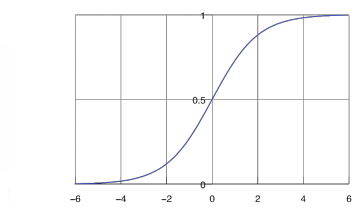
\includegraphics[width=0.5\textwidth]{fig/FonctionSigm.png}
	\caption{Fonction Sigmoïde}
	\label{fig:image4}
\end{figure} \\
On remarque que cette fonction ne prend que des valeurs comprise entre 0 et 1.

En d'autres termes ${h}_{\theta}\left(x\right)$ représente la probabilité que y=1 sur l'entrée  ${x}_{n}$ .
\begin{center}
	${h}_{\theta}\left(x\right)=P(y=1|x;\theta)$
\end{center}
La probabilité que y soit égale à 1 sachant ${x}_{n}$ paramétré par $\theta$.

On l'utilise pour effectuer une classification en supposant que :

- si ${h}_{\theta}\left(x\right)> 0.5 $ la classe prédite est 1.

- si ${h}_{\theta}\left(x\right)< 0.5 $ la classe prédite est 0.

On démontre que :
\begin{center}
	$P(y=1|x;\theta) + P(y=0|x;\theta) = 1 $ et
	
	$P(y=0|x;\theta) = 1-  P(y=1|x;\theta)$
\end{center}
\subsubsection{Frontière de Décision }
Analysons notre fonction $g(z)$ , on remarque qu'il est égale à 0.5 pour z = 0.
Donc si z est positif $g(z)$ sera supérieur à 0.5, dans le cas contraire $g(z)$ sera inférieur à 0.5.
Et ainsi avec notre hypothèse
$h({\theta }^{T}{x}) = 1 $ si  ${\theta }^{T}{x}$ > 0 et 
$h({\theta }^{T}{x}) = 0 $ si  ${\theta }^{T}{x}$ < 0
On comprend qu'a partir du plan  ${\theta }^{T}{x}$ qui divise l'espace en 2 partie on peut prédire la classe de chaque tuple  sans problème .

Cette droite ou hyperplan  s'appelle \emph{\textbf{la frontière de décision }}.
Voici comment elle se présente si on n'a que 2 attributs ${x}_{1}$ et ${x}_{2}$ :
\begin{figure}[ht]
	\centering
	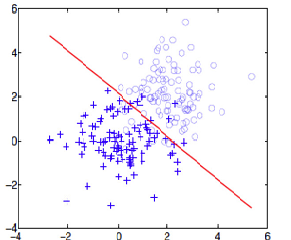
\includegraphics[width=0.5\textwidth]{fig/DecisionBoudary.png}
	\caption{Frontière de décision pour la Régression Logistique à 2 variables}
	\label{fig:image5}
\end{figure}

\subsubsection{La Fonction Coût : Calcul De L'erreur }

On pourrait être tenter d'utiliser la même fonction coût que pour la régression linéaire 

\begin{center}
	 $J\left({\theta }_{1},{\theta }_{2},.....{\theta }_{n}\right)=\frac{1}{2m}\sum _{=1}^{m}{\left[{h}_{\theta}\left({x}^{(i)}\right) - {y}^{(i)}\right]}^2$
\end{center}
Mais cette fonction présente des problèmes de convergence à cause de la non linéarité de la fonction ${h}_{\theta}\left(x\right)$.
Pour ce faire,on définit une nouvelle fonction de l'erreur:

$Err({h}_{\theta}\left(x\right),y) = \left\{\begin{array}{ll}
-\log [1-{h}_{\theta}\left(x\right)], & \mbox{si } y\mbox{=0}   \\
-\log [{h}_{\theta}\left(x\right)], & \mbox{si } y\mbox{=1} 
\end{array}\right.$

\emph{\textbf{Analyse de l'erreur :}}

- si y= 1 et notre fonction ${h}_{\theta}\left(x\right)=1$, alors l'erreur vaut 0 et augmente si  ${h}_{\theta}\left(x\right)$ décroit.

- si y= 0 et notre fonction ${h}_{\theta}\left(x\right)=0$, alors l'erreur vaut 0 et augmente si  ${h}_{\theta}\left(x\right)$ croit . 

On peut facilement le remarquer sur les figures suivantes: \\
\begin{figure}[ht]
	\centering
	\subfloat[cas ou Y =1]{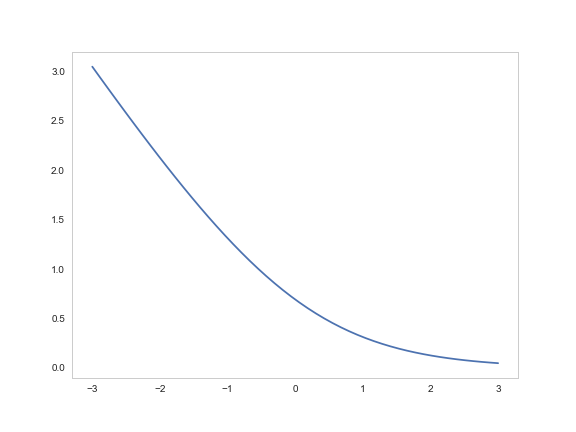
\includegraphics[width=0.4\textwidth]{fig/ErreurRegressionLogistique.png}\label{fig:Image6a}}
	\hfill
	\subfloat[Y = 0]{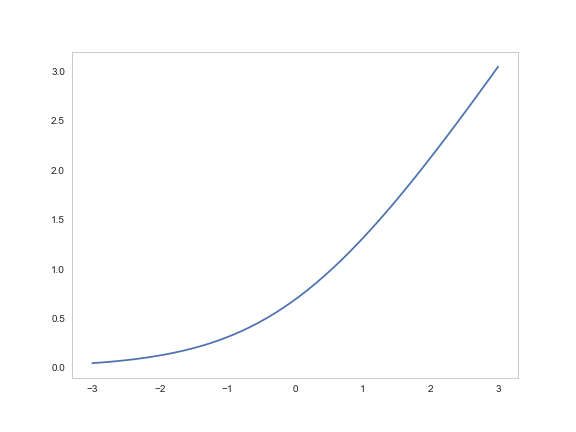
\includegraphics[width=0.4\textwidth]{fig/ErreurRegressionLogistique2.png}\label{fig:Image6b}}
	\hfill
	\caption{Erreur  pour la régression logistique}
\end{figure}
Notre fonction cout peut prendre la forme compacte suivante :
\begin{center}
	$Err({h}_{\theta}\left(x\right),y) = -y\log [{h}_{\theta}\left(x\right)] -(1-y)\log [1-{h}_{\theta}\left(x\right)]$ 
\end{center}	
Et Donc notre Fonction cout pour les $\theta$ sera :
\begin{center}
$J\left({\theta }\right)=\frac{1}{2m}[\sum _{=1}^{m}-{y}^{(i)}\log [{h}_{\theta}\left({x}^{(i)}\right)] -(1-{y}^{(i)})\log [1-{h}_{\theta}\left({x}^{(i)}\right)]]$
\end{center}


Avec ${h}_{\theta}\left(x\right) =\frac{1}{1+{e}^{-{\theta }^{T}{x}}}$

 Pour le minimiser,on recours aux mêmes techniques que pour la régression linéaire et c'est le même algorithme de la descente du gradient qu'on utilise  dans ce cas aussi.
\subsubsection{Régulation : Phénomène de sur-apprentissage}
Nous venons de passer en revue quelques modèles pour  effectuer la régression linéaire ainsi que la classification avec la régression logistique.
Jetons un coup d'œil aux 3 images de la `\figurename{ 7 }  \\
\begin{figure}[ht]
	\centering
	\subfloat[${h}_{\theta}\left(x\right)={\theta }_{0}+{\theta }_{1}x$]{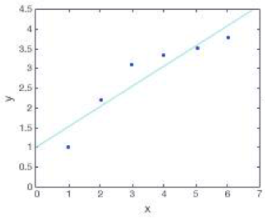
\includegraphics[width=0.4\textwidth]{fig/Overfiitting1.png}\label{fig:Image7a}}
	\hfill
	\subfloat[${h}_{\theta}\left(x\right)={\theta }_{0}+{\theta }_{1}x+{\theta }_{2}{x}^{2}$]{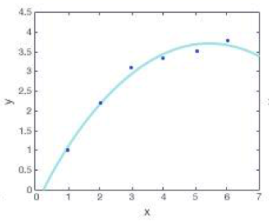
\includegraphics[width=0.4\textwidth]{fig/Overfiitting2.png}\label{fig:Image7b}}
	\hfill
	\subfloat[${h}_{\theta}\left(x\right)={\theta }_{0}+{\theta }_{1}x+{\theta }_{2}{x}^{2}+{\theta }_{3}{x}^{3}+{\theta }_{4}{x}^{4}$]{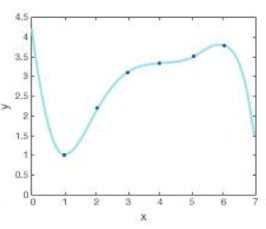
\includegraphics[width=0.4\textwidth]{fig/Overfiitting3.png}\label{fig:Image7c}}
	\caption{a: Sous-apprentissage et c : Sur-apprentissage avec la régression linéaire}
\end{figure}
A la première figure (a) : avons la régression linéaire comme hypothèse  mais on remarque que cela n'est pas un bon modèle de prédiction car dans ce cas l'erreur est trop grande.on parle de \emph{sous-apprentissage ou Underfitting}.
A la deuxième figure notre hypothèse c'est un polynôme du second dégrée le modèle convient bien à notre ensemble d'apprentissage et dans ce cas l'erreur est moins élevée.
Par contre sur la troisième cas l'hypothèse c'est un polynôme du quatrième dégrée qui convient parfaitement à notre ensemble d'apprentissage et l'erreur est nulle, mais c'est modèle n'est pas bon  car il  convient parfaitement sur notre ensemble d'apprentissage et n'est pas adaptable aux nouvelles données, elle n'est pas une solution générale.Dans ce cas on parle de \emph{Sur-Apprentissage ou Overfitting } .

On remarque ce même phénomène avec la régression logistique .

\begin{figure}[H]
	\centering
	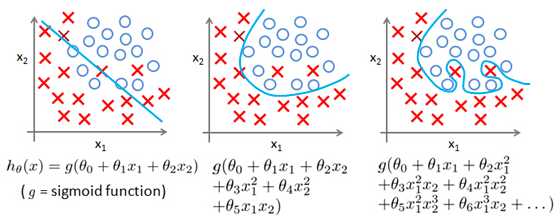
\includegraphics[width=0.5\textwidth]{fig/OverfiittingLogistic.png}
	\caption{Overfitting et Underfitting avec la régression logistique }
	\label{fig:image8}
\end{figure}
\subsubsection{Solutions aux problèmes de sur apprentissage }
Signalons qu'une des cause de ce phénomène c'est le fait d'avoir peut des données avec plusieurs attributs .

Dans ce cas la première de solution consisterait à réduire le nombre des attribues , choisir celle qu'on doit retenir et laisser les autres,mais cette approche possède un inconvénient car on risquerait de perdre l'information apportée par ces attributs et cela pénaliserait notre modèle .

La seconde solution est celle qu'on appelle la \emph{La régularisation } elle consiste à garde tous les attributs mais réduire l'ampleur des paramètres  $\theta$ dans le calcul de l'erreur . On remarque que cette technique fonctionne très bien lorsqu'on dispose de plusieurs attributs qui contribue à la prédiction de la valeur y.
Ainsi notre fonction de cout pour le calcul de l'erreur de la régression linéaire sera :

\begin{center}
	$J\left({\theta }_{1},{\theta }_{2},.....{\theta }_{n}\right)=\frac{1}{2m}[\sum _{=1}^{m}{\left[{h}_{\theta}\left({x}^{(i)}\right) - {y}^{(i)}\right]}^{2} + {\lambda} \sum _{=1}^{n}{{\theta}_{j}^{2}}]$
\end{center}
Et Pour la régression logistique elle sera :

\begin{center}
	$J\left({\theta }\right)=\frac{1}{2m}[\sum _{=1}^{m}-{y}^{(i)}\log [{h}_{\theta}\left({x}^{(i)}\right)] -(1-{y}^{(i)})\log [1-{h}_{\theta}\left({x}^{(i)}\right)] + {\lambda} \sum _{=1}^{n}{{\theta}_{j}^{2}}]$
\end{center}

Avec $\lambda$ le facteur de régularisation. 
C'est cette nouvelle fonction cout qu'on utilise pour l'algorithme de la descente du gradient régularisé.\\ 
